\documentclass[11pt,a4paper,titlepage]{article}
\usepackage[a4paper]{geometry}
\usepackage[utf8]{inputenc}
\usepackage[english]{babel}
\usepackage{lipsum}

\usepackage{amsmath, amssymb, amsfonts, amsthm, fouriernc, mathtools}
% mathtools for: Aboxed (put box on last equation in align envirenment)
\usepackage{microtype} %improves the spacing between words and letters

\usepackage{graphicx,float}
\graphicspath{ {./pics/} {./eps/}}
\usepackage{epsfig}
\usepackage{epstopdf}


%%%%%%%%%%%%%%%%%%%%%%%%%%%%%%%%%%%%%%%%%%%%%%%%%%
%% COLOR DEFINITIONS
%%%%%%%%%%%%%%%%%%%%%%%%%%%%%%%%%%%%%%%%%%%%%%%%%%
\usepackage[svgnames]{xcolor} % Enabling mixing colors and color's call by 'svgnames'
%%%%%%%%%%%%%%%%%%%%%%%%%%%%%%%%%%%%%%%%%%%%%%%%%%
\definecolor{MyColor1}{rgb}{0.2,0.4,0.6} %mix personal color
\newcommand{\textb}{\color{Black} \usefont{OT1}{lmss}{m}{n}}
\newcommand{\blue}{\color{MyColor1} \usefont{OT1}{lmss}{m}{n}}
\newcommand{\blueb}{\color{MyColor1} \usefont{OT1}{lmss}{b}{n}}
\newcommand{\red}{\color{LightCoral} \usefont{OT1}{lmss}{m}{n}}
\newcommand{\green}{\color{Turquoise} \usefont{OT1}{lmss}{m}{n}}
%%%%%%%%%%%%%%%%%%%%%%%%%%%%%%%%%%%%%%%%%%%%%%%%%%




%%%%%%%%%%%%%%%%%%%%%%%%%%%%%%%%%%%%%%%%%%%%%%%%%%
%% FONTS AND COLORS
%%%%%%%%%%%%%%%%%%%%%%%%%%%%%%%%%%%%%%%%%%%%%%%%%%
%    SECTIONS
%%%%%%%%%%%%%%%%%%%%%%%%%%%%%%%%%%%%%%%%%%%%%%%%%%
\usepackage{titlesec}
\usepackage{sectsty}
%%%%%%%%%%%%%%%%%%%%%%%%
%set section/subsections HEADINGS font and color
\sectionfont{\color{MyColor1}}  % sets colour of sections
\subsectionfont{\color{MyColor1}}  % sets colour of sections
\subsubsectionfont{\color{MyColor1}}
\paragraphfont{\color{MyColor1}}
\subparagraphfont{\color{MyColor1}}

%set section enumerator to arabic number (see footnotes markings alternatives)
\renewcommand\thesection{\arabic{section}.} %define sections numbering
\renewcommand\thesubsection{\thesection\arabic{subsection}} %subsec.num.

%define new section style
\newcommand{\mysection}{
\titleformat{\section} [runin] {\usefont{OT1}{lmss}{b}{n}\color{MyColor1}} 
{\thesection} {3pt} {} } 

%%%%%%%%%%%%%%%%%%%%%%%%%%%%%%%%%%%%%%%%%%%%%%%%%%
%		CAPTIONS
%%%%%%%%%%%%%%%%%%%%%%%%%%%%%%%%%%%%%%%%%%%%%%%%%%
\usepackage{caption}
\usepackage{subcaption}
%%%%%%%%%%%%%%%%%%%%%%%%
\captionsetup[figure]{labelfont={color=Blue}}

%%%%%%%%%%%%%%%%%%%%%%%%%%%%%%%%%%%%%%%%%%%%%%%%%%
%		!!!EQUATION (ARRAY) --> USING ALIGN INSTEAD
%%%%%%%%%%%%%%%%%%%%%%%%%%%%%%%%%%%%%%%%%%%%%%%%%%
%using amsmath package to redefine eq. numeration (1.1, 1.2, ...) 
%%%%%%%%%%%%%%%%%%%%%%%%
\renewcommand{\theequation}{\thesection\arabic{equation}}

%set box background to grey in align environment 
\usepackage{etoolbox}% http://ctan.org/pkg/etoolbox
\makeatletter
\patchcmd{\@Aboxed}{\boxed{#1#2}}{\colorbox{black!15}{$#1#2$}}{}{}%
\patchcmd{\@boxed}{\boxed{#1#2}}{\colorbox{black!15}{$#1#2$}}{}{}%
\makeatother
%%%%%%%%%%%%%%%%%%%%%%%%%%%%%%%%%%%%%%%%%%%%%%%%%%




%%%%%%%%%%%%%%%%%%%%%%%%%%%%%%%%%%%%%%%%%%%%%%%%%%
%% DESIGN CIRCUITS
%%%%%%%%%%%%%%%%%%%%%%%%%%%%%%%%%%%%%%%%%%%%%%%%%%
\usepackage[siunitx, american, smartlabels, cute inductors, europeanvoltages]{circuitikz}
%%%%%%%%%%%%%%%%%%%%%%%%%%%%%%%%%%%%%%%%%%%%%%%%%%



\makeatletter
\let\reftagform@=\tagform@
\def\tagform@#1{\maketag@@@{(\ignorespaces\textcolor{red}{#1}\unskip\@@italiccorr)}}
\renewcommand{\eqref}[1]{\textup{\reftagform@{\ref{#1}}}}
\makeatother
\usepackage{hyperref}
\hypersetup{colorlinks=true}

%%%%%%%%%%%%%%%%%%%%%%%%%%%%%%%%%%%%%%%%%%%%%%%%%%
%% PREPARE TITLE
%%%%%%%%%%%%%%%%%%%%%%%%%%%%%%%%%%%%%%%%%%%%%%%%%%
\title{\blue Software Design Description  \\
\blueb StreamCam}
\author{Juan S. Carrillo Quinche}
\date{\today}
%%%%%%%%%%%%%%%%%%%%%%%%%%%%%%%%%%%%%%%%%%%%%%%%%%



\begin{document}
\maketitle

\section{Scope}
\section{Referenced Documents}
\section{Requirements}
\section{Architectural Design}
\subsection{CSCI Architectural Design}
\subsection{CSCI Components}
\subsection{Concept of Execution}
\subsection{Interface Design}
\subsubsection{Interface Identification and Diagrams}
\subsubsection{Project-unique Identifier and Interface}
\subsubsection{Project Interactions}
\paragraph{Directory Structure}
\paragraph{Startup Control}
\section{CSCI Detailed Design}
\subsection{CSC 1 Detailed Design}
\subsection{CSC $n$ Detailed Design}
\subsection{Hardware Interfacing}
\subsection{Intra-Level Processing and Data Transfer}
\subsection{Unit Test Scripts}

%%%%% SDD GOES HERE
\section{Requirements Traceability}
\subsection{Introduction}
Stream Cam is an Android application that will allow users to record and simultaneously stream videos to a remote database. Users can manage their videos on the database via a desktop web client.
\subsubsection{System Objectives}
The goal of StreamCam is to provide users a way to safely store videos that they record on their phones. By streaming their videos to a remote database, users can be sure that even if their phones are damaged or destroyed or confiscated their videos will remain saved. 

Each video can have an associated location manifest which provides the user's location during the time the video was recorded. This is done in hopes that if user's need to provide legal evidence to support their account of a traffic accident, for example. 

StreamCam should be able to handle losing connection to the database by streaming the stored video as soon as it gets internet connection. 

Users will be able to manage their videos through a web client, which will provide a simple interface for them to manage and download their videos in the database. 

\subsubsection{Interfaces}

The Android phone will communicate with the server in one of two ways. The client can provide server with HTTP requests for actions such as login, creating new users, or notifying the server that the phone is about to stream a video to the server. The Android phone will act as an RTP server to stream videos to the  remote server, which will request the video stream from the client. 

\subparagraph{StreamCam API\\}

The Android client will communicate with the StreamCam API and make general requests and authorized requests. General requests can be done by anyone, and they include login and creating new accounts. Authorized requests require that the user be signed in to StreamCam. Once they have been authorized through the use of web tokens, users can perform authorized requests. 
\begin{enumerate}
  \item The Android client can notify the server if the phone is about to start or end a stream.
  \item The Android client can post the user's location when recording a video. 
  \item The web client can request to view a listing of the user's videos.
  \item The web client can request to download a user's videos.
  \item The web client can request to delete a user's videos.
\end{enumerate}

\subparagraph{Server-Database Interface\\}

I make use the \textbf{pg} Node library, which allows me to write server-side CoffeeScript that interface with the database. 

\subsection{Architectural Design}

My system will use a simple three-tier architecture. It will constist of clients, a server that will handle all the logic and requests from users, and a database that will store user information. 

I have a three-tier architecture with three different servers that are used for specialized purposes. I have used a github server to host the web client. I have used an Amazon EC2 server to host the Wowza Streaming Engine, which allows users to stream their videos from their phones to the server. I also have a Heroku server which manages users and videos. This Heroku server is the central hub, as it handles all the logic from the clients and interfaces with the Amazon server to work with the streaming services. 

\subsubsection{Major Software Components}
The major software components can be broken down into Android Client, Web Client, and Server. 

\paragraph{Android Client\\}
    The Android client is the most complex component. It consists of three to five activities or screens that the user will interact with directly, as well as internal logic which will handle creating requests as well as streaming video to the server.
    
    The activities will include a login screen, a create account screen, a camera screen, a settings screen, and possibly a video manager screen. The login screens and create account screens will be minimal, and will be the standard run of the mill login and create account screens. For now, StreamCam will not allow users to recover their accounts. This feature will be added if time permits. The Camera Screen is where the user will spend the majority of their time. It will present what the camera is capturing and will have a simple button to start and pause streaming. The settings screen will allow the users to manage their settings, such as whether or not they want the camera to remain on when they pause StreamCam(useful for recording while using another app such as a GPS). Finally, time permitting StreamCam will include a screen that will allow users to manage their videos.
    
    
    The Android client will keep track of the user's location and send this information to the server. This feature is not enabled by default; the user must enable this feature. The Android client will have logic that will allow the phone to continue streaming video after an internet service interruption.
    
\paragraph{Web Client\\}
	The web client is the simplest component. The web client will allow users to login or create an account. When a user logs in they will have a simple screen similar to the view of a standard file management system that will allow users to manage and download their stored videos. Each file will have information such as duration, the date the video was recorded, and a text file that provides the user's location during the duration of the video. If the user did not enable this feature, the location manifest will not be present. 
	
\paragraph{Server\\}
    The server has moderate complexity. The server will handle all client requests from Android and Web Clients and interact with the database to give users the information they require. 
    
\subsubsection{Major Software Interactions}

\paragraph{User Login and Creating New Accounts\\}
This interaction is between the Android Client or the Web Client and the server. During this interaction the user will either create a new account or provide credentials for an existing account. After doing either successfully the user will receive a token that will allow them to perform other actions.

\paragraph{Streaming\\}
I'm still trying to figure out how to implement this.

\paragraph{Viewing User Videos\\}
The web client will be able to make requests to the StreamCam server to view all the users videos. It will receive a list of videos with basic information such as duration, date the video was recorded, and a link to download the video. The user will also have the ability to delete videos that they have recorded.

\subsubsection{Architectural Design Diagrams}

\begin{figure}[H]
  \centering
  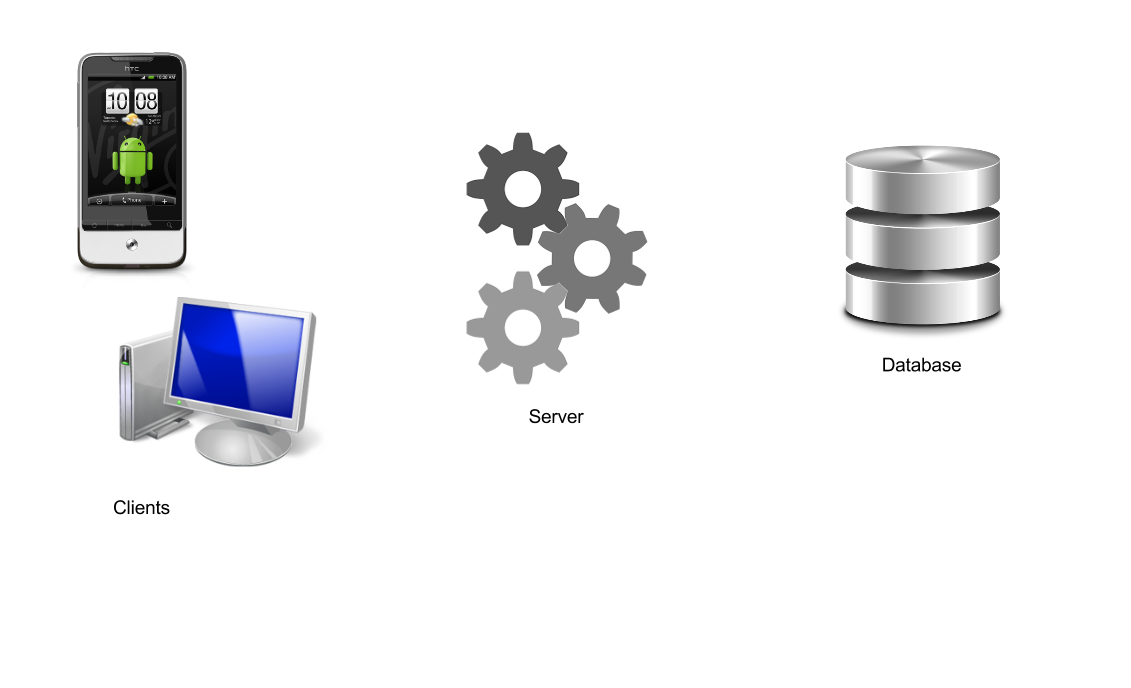
\includegraphics[width=0.8\textwidth]{img/architecture.png}
  \caption{Figure of Architecture}
\end{figure}

Below is a figure that explains the streaming architecture.

\begin{figure}[H]
  \centering
  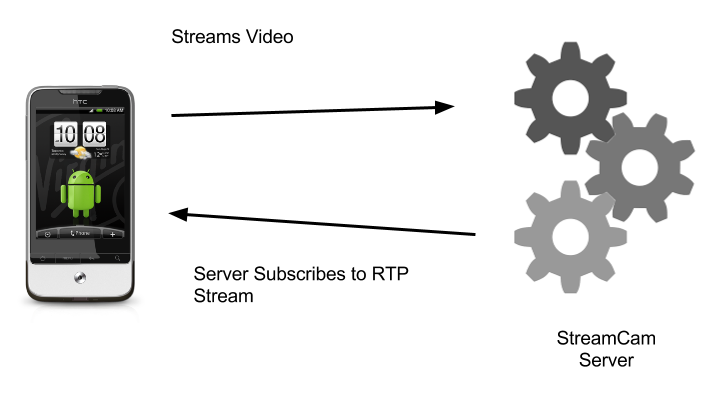
\includegraphics[width=5in]{img/streaming-architecture.png}
  \caption{Figure of Architecture}
\end{figure}

Below is a use case diagram for streaming.

\begin{figure}[H]
  \centering
  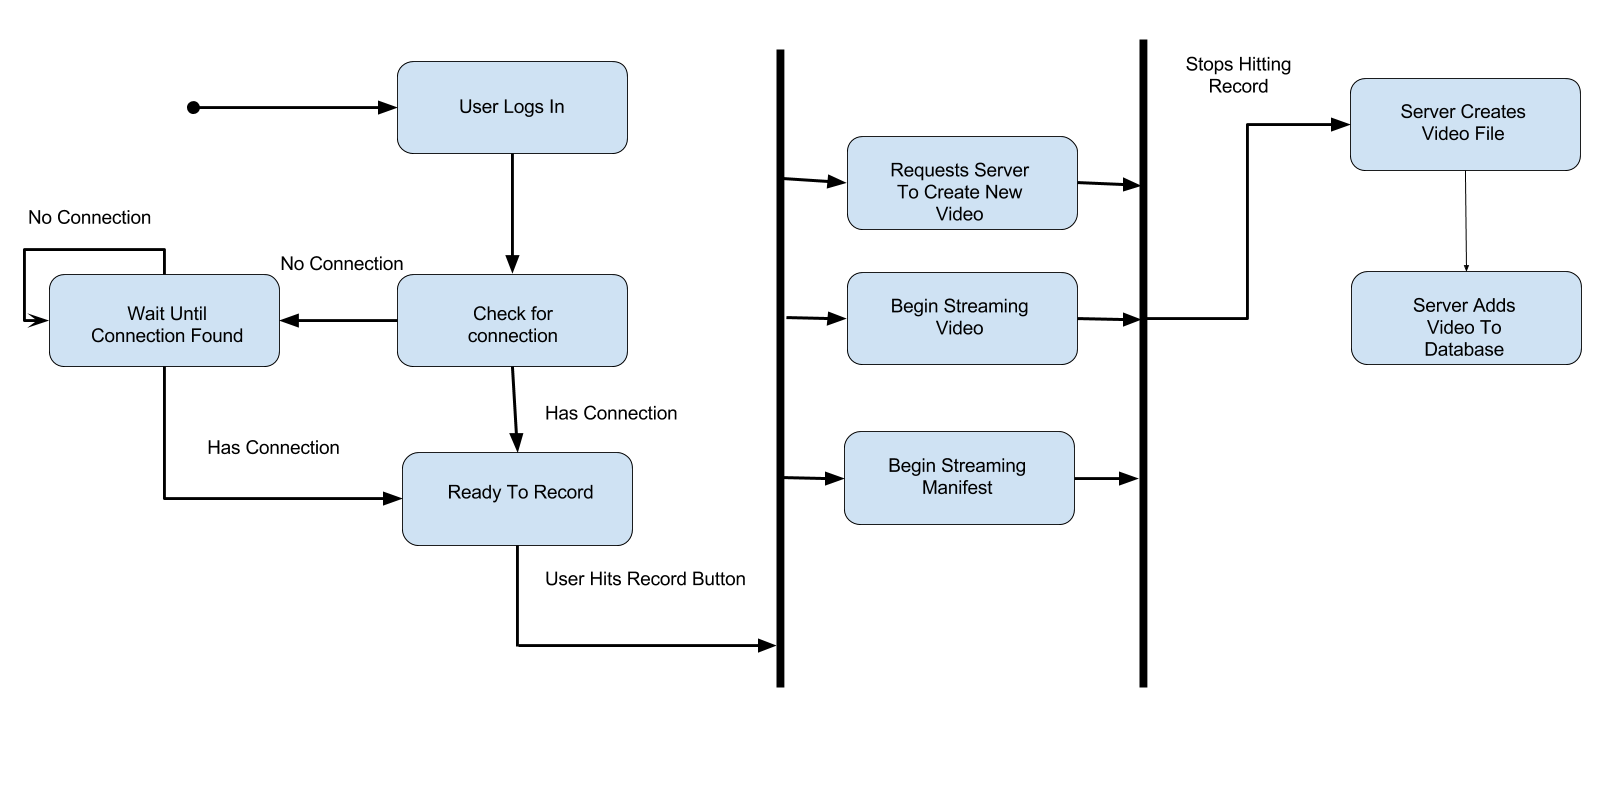
\includegraphics[width=5in]{img/uml_streaming.png}
  \caption{Figure of Architecture}
\end{figure}

Below is a UML diagram of classes used for the Android Client.

\begin{figure}[H]
  \centering
  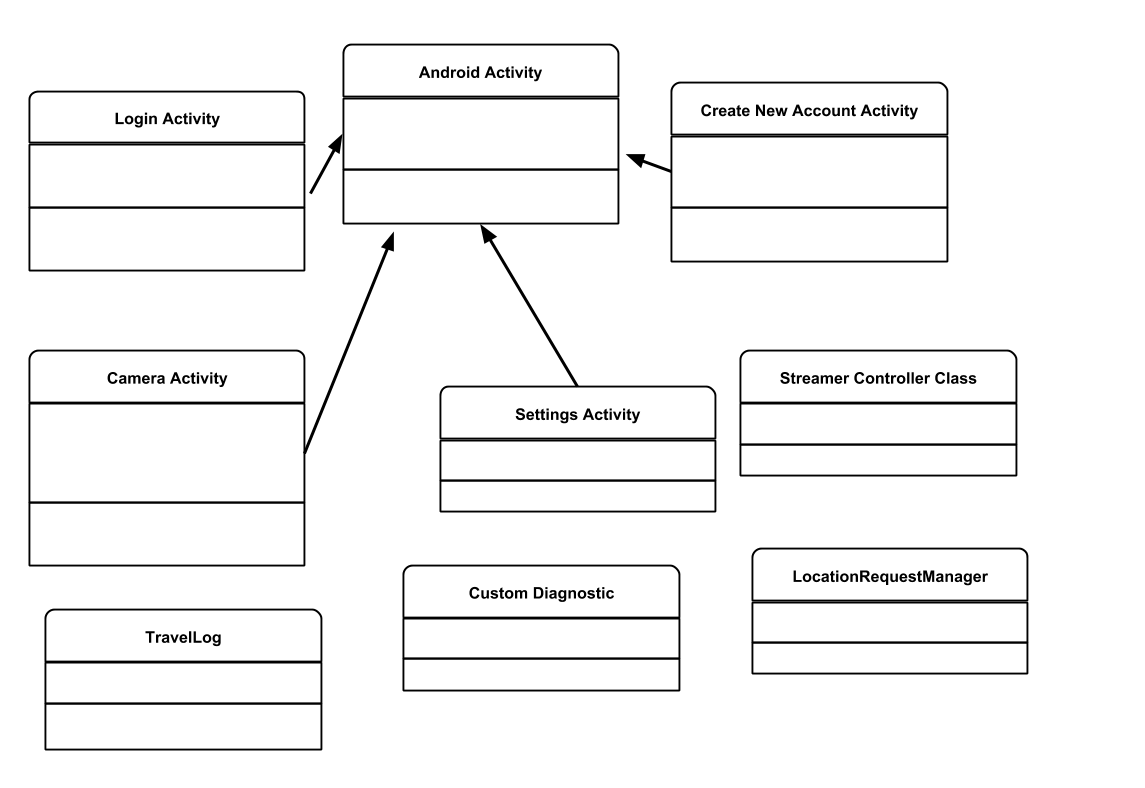
\includegraphics[width=5in]{img/android_classes}
  \caption{Figure of Architecture}
\end{figure}



\subsection{CSC and CSU Descriptions}
I have server side code, Android client code, and web client code. The most complex is the Android client.  Android screens are classes called activities. Each of these has code that contains the functionality for the screen that the user will interact with at that particular part of the phone app. All of them inherit methods from the Activity class. The Activity class has basic methods such as onCreate, onPause, and onEnd that specify what is done when a particular screen is created, paused, or destroyed. I will focus on the functionality of each screen.

\subsubsection{Class Descriptions}
The following are class descriptions for the Android client.
\paragraph{Login Activity\\}
The login activity is a simply screen with text fields for users to enter their username and password. It also has two buttons: one for login in and the other to go to the Create Account Screen. The Login Screen has very few fields and methods.
\\

\textbf{FIELDS}
\begin{enumerate}
  \item mUsername - (String) Stores the provided username.
  \item mUsernameTextView - (TextView) A reference to the input field where the user provides their username.
  \item mPassword - (String) Stores the provided password.
  \item mPasswordTextView - (TextView) A reference to the input field where the user provides their password.
\end{enumerate}

\textbf{METHODS}
\begin{enumerate}
  \item onCreate - void. Setups the activity.
  \item onLoginButtonClicked - void. Handles logic for when login button is clicked.
  \item goToCameraActivity - void. Used to go to the Camera Activity.
  \item goToCreateAccountActivity - void. User to go to the Create Account Activity.
  \item handleHTTPResponse - void. Handles HTTP response from server.
\end{enumerate}

\paragraph{Create Account Activity\\}
This activity is a simply screen with text fields for users to enter their username and password. It also has one button that is used to submit data to create a new account. There are three textfields, one for a user name and two for the password. The second textfield is used to confirm the user's password.
\\

\textbf{FIELDS}
\begin{enumerate}
  \item mUsername - (String) Stores the provided username.
  \item mUsernameTextView - (TextView) A reference to the input field where the user provides their username.
  \item mPassword - (String) Stores the provided password.
  \item mPasswordTextView - (TextView) A reference to the input field where the user provides their password.
  \item mPasswordConfirm - (String) Stores the provided confirm password.
  \item mPasswordConfirmTextView - (TextView) A reference to the input field where the user provides their confirm password.
\end{enumerate}

\textbf{METHODS}
\begin{enumerate}
  \item onCreate - void. Setups the activity.
  \item onCreateAccountButtonClicked - void. Handles logic for when login button is clicked.
  \item goToCameraActivity - void. Used to go to the Camera Activity.
  \item handleHTTPResponse - void. Handles HTTP response from server.
\end{enumerate}

\paragraph{Camera Activity\\}
This activity is the most complex. It is not yet fully implemented. It has the necessary code to show the camera screen and retrieve the user's current location.

The following are class descriptions for server.

\paragraph{server.coffee\\}
This class is the server that the Android client will communicate with. This class will not have any logic, rather, it will set up the routes for the API. 

\paragraph{login.coffee\\}
This class has the logic for login in and creating new users. It has just two methods, loginUser and createNewUser. Both of these return a JSON response that will be parsed by the JSON client.

\textbf{METHODS}
\begin{enumerate}
  \item loginUser - Takes in an HTTP request variable. Returns an HTTP response. It checks that the login credentials provided in the request body are valid, and if so provides the user with a web token.
  \item createNewUser - Takes in an HTTP request variable. Returns an HTTP response. It checks that the username provided by the user is available, and if so creates an account and returns a web token with the response.
\end{enumerate}

\paragraph{token.coffee\\}
This class stores the JSON web tokens that are created to authenticate users. It has two methods, createToken and decodeToken. While this functionality could be included in some other class, it makes sense to separate the tokens in their own class for separation of concerns.

\textbf{METHODS}
\begin{enumerate}
  \item createToken - Takes in a username. Returns a web token. 
  \item decodeToken - Takes in a web token. Returns a decoded web token for the use of the server to authenticate the user.
\end{enumerate}

\paragraph{manifest.coffee\\}
This class has the logic that deals with the video manifest. It has code for appending to the manifest in the database, creating a string representation of the manifest, and returning manifests for a particular video. Not implemented completely.

\paragraph{stream.coffee\\}
This class has the logic for creating threads to listen to users' streams. No idea how to do this yet.


\subsubsection{Detailed Interface Descriptions}
The interfaces for my project are my server and the middleware routes.
\subsubsection{Detailed Data Structure Descriptions}
The manifest, which is not fully implemented, is a linked list. Since we will constantly be appending to the manifest, I chose a linked list because we avoid having to resize the array. The manifest will have a pointer to the current location. This allows us to keep track of which location has been sent to the server so we can send locations in chronological order. 
\subsubsection{Detailed Design Diagrams}
Please refer to architecture section for diagrams.
\subsection{Database Design and Description}
The database contains information about users and their videos. It stores user credentials, information about videos, including duration, date, and a manifest with the user's location at the time the video was made.

There is a one-to-many correspondence between users and videos. Each user can have many videos, and a video is owned by a single user. There is a one-to-one correspondence between a video and a manifest. Each video has a single manifest, and a manifest belongs to a single video.

\subsubsection{Database Design ER Diagram}
\begin{figure}[H]
  \centering
  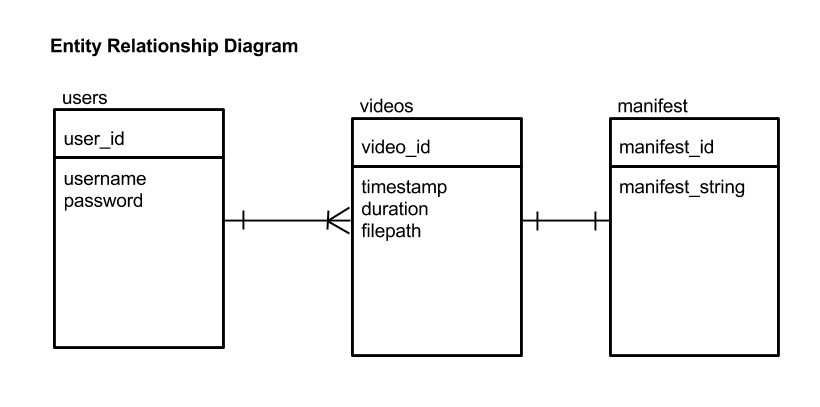
\includegraphics[width=5in]{img/erd.png}
  \caption{Figure of Architecture}
\end{figure}
\subsubsection{Database Access}
As of now only the server is the sole user of the database. 
\subsubsection{Database Security}
As of now only the server is the sole user of the database. I will have to provide additional security features later.
%%%%% SDD ENDS HERE
\section{Notes}
\section{Acronyms and Abbreviations}


\end{document}